% Architecture of doc_manager (original code, commit 5943319): who talks to whom.
\documentclass[border=8pt]{standalone}
\usepackage{tikz}
% Shared look for all diagrams. Grey = Django class, blue = app class, green = added in Part 2.
\usetikzlibrary{positioning,shapes.multipart,arrows.meta,fit,backgrounds}
\definecolor{djangoC}{HTML}{E6E6E6}
\definecolor{appC}{HTML}{D6E8FA}
\definecolor{newC}{HTML}{D5F0D5}
\newcommand{\role}[1]{{\footnotesize\itshape #1}}
\tikzset{
  box/.style={draw, rectangle split, rectangle split parts=2, align=center,
              font=\small, inner sep=5pt, minimum width=3.6cm},
  djcls/.style={box, rectangle split part fill={djangoC,white}},
  appcls/.style={box, rectangle split part fill={appC,white}},
  newcls/.style={box, rectangle split part fill={newC,white}},
  plain/.style={draw, align=center, font=\small, inner sep=5pt, minimum width=3.2cm, minimum height=1cm},
  note/.style={draw, align=left, font=\footnotesize, fill=yellow!12, inner sep=4pt},
  inherits/.style={-{Triangle[open,length=3mm,width=3mm]}, thick},
  uses/.style={-{Stealth[length=2.5mm]}, thick},
  lbl/.style={font=\footnotesize, fill=white, inner sep=1.5pt},
  num/.style={circle, draw, fill=white, font=\scriptsize\bfseries, inner sep=1.2pt},
}

\begin{document}
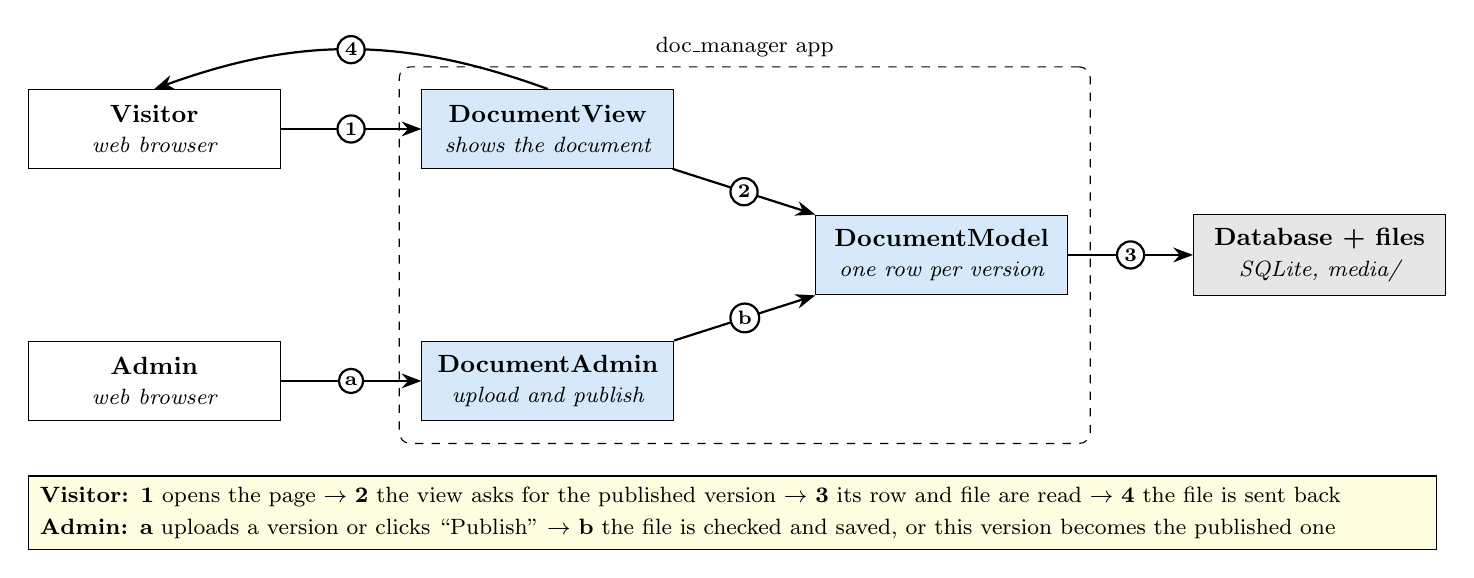
\begin{tikzpicture}
\node[plain] (visitor) at (0, 1.6)  {\textbf{Visitor}\\ \role{web browser}};
\node[plain] (admin)   at (0,-1.6)  {\textbf{Admin}\\ \role{web browser}};
\node[plain, fill=appC] (view)  at (5, 1.6)  {\textbf{DocumentView}\\ \role{shows the document}};
\node[plain, fill=appC] (adm)   at (5,-1.6)  {\textbf{DocumentAdmin}\\ \role{upload and publish}};
\node[plain, fill=appC] (model) at (10, 0)   {\textbf{DocumentModel}\\ \role{one row per version}};
\node[plain, fill=djangoC] (db) at (14.8, 0)   {\textbf{Database + files}\\ \role{SQLite, media/}};
\begin{scope}[on background layer]
  \node[draw, dashed, rounded corners, fit=(view)(adm)(model), inner sep=8pt,
        label={[font=\footnotesize]above:doc\_manager app}] {};
\end{scope}
\draw[uses] (visitor) -- node[num] {1} (view);
\draw[uses] (view) -- node[num] {2} (model);
\draw[uses] (model) -- node[num] {3} (db);
\draw[uses] (view.north) to[out=160, in=20] node[num] {4} (visitor.north);
\draw[uses] (admin) -- node[num] {a} (adm);
\draw[uses] (adm) -- node[num] {b} (model);
\node[note, anchor=north west, text width=17.6cm] at (-1.6,-2.8)
 {\textbf{Visitor:} \textbf{1} opens the page $\rightarrow$ \textbf{2} the view asks for the published version
  $\rightarrow$ \textbf{3} its row and file are read $\rightarrow$ \textbf{4} the file is sent back\\[2pt]
  \textbf{Admin:} \textbf{a} uploads a version or clicks ``Publish'' $\rightarrow$ \textbf{b} the file is checked and
  saved, or this version becomes the published one};
\end{tikzpicture}
\end{document}
